\documentclass[11pt,preprint, authoryear]{elsarticle}

\usepackage{lmodern}
%%%% My spacing
\usepackage{setspace}
\setstretch{1.2}
\DeclareMathSizes{12}{14}{10}{10}

% Wrap around which gives all figures included the [H] command, or places it "here". This can be tedious to code in Rmarkdown.
\usepackage{float}
\let\origfigure\figure
\let\endorigfigure\endfigure
\renewenvironment{figure}[1][2] {
    \expandafter\origfigure\expandafter[H]
} {
    \endorigfigure
}

\let\origtable\table
\let\endorigtable\endtable
\renewenvironment{table}[1][2] {
    \expandafter\origtable\expandafter[H]
} {
    \endorigtable
}


\usepackage{ifxetex,ifluatex}
\usepackage{fixltx2e} % provides \textsubscript
\ifnum 0\ifxetex 1\fi\ifluatex 1\fi=0 % if pdftex
  \usepackage[T1]{fontenc}
  \usepackage[utf8]{inputenc}
\else % if luatex or xelatex
  \ifxetex
    \usepackage{mathspec}
    \usepackage{xltxtra,xunicode}
  \else
    \usepackage{fontspec}
  \fi
  \defaultfontfeatures{Mapping=tex-text,Scale=MatchLowercase}
  \newcommand{\euro}{€}
\fi

\usepackage{amssymb, amsmath, amsthm, amsfonts}

\def\bibsection{\section*{References}} %%% Make "References" appear before bibliography


\usepackage[round]{natbib}

\usepackage{longtable}
\usepackage[margin=2.3cm,bottom=2cm,top=2.5cm, includefoot]{geometry}
\usepackage{fancyhdr}
\usepackage[bottom, hang, flushmargin]{footmisc}
\usepackage{graphicx}
\numberwithin{equation}{section}
\numberwithin{figure}{section}
\numberwithin{table}{section}
\setlength{\parindent}{0cm}
\setlength{\parskip}{1.3ex plus 0.5ex minus 0.3ex}
\usepackage{textcomp}
\renewcommand{\headrulewidth}{0.2pt}
\renewcommand{\footrulewidth}{0.3pt}

\usepackage{array}
\newcolumntype{x}[1]{>{\centering\arraybackslash\hspace{0pt}}p{#1}}

%%%%  Remove the "preprint submitted to" part. Don't worry about this either, it just looks better without it:
\makeatletter
\def\ps@pprintTitle{%
  \let\@oddhead\@empty
  \let\@evenhead\@empty
  \let\@oddfoot\@empty
  \let\@evenfoot\@oddfoot
}
\makeatother

 \def\tightlist{} % This allows for subbullets!

\usepackage{hyperref}
\hypersetup{breaklinks=true,
            bookmarks=true,
            colorlinks=true,
            citecolor=blue,
            urlcolor=blue,
            linkcolor=blue,
            pdfborder={0 0 0}}


% The following packages allow huxtable to work:
\usepackage{siunitx}
\usepackage{multirow}
\usepackage{hhline}
\usepackage{calc}
\usepackage{tabularx}
\usepackage{booktabs}
\usepackage{caption}


\newenvironment{columns}[1][]{}{}

\newenvironment{column}[1]{\begin{minipage}{#1}\ignorespaces}{%
\end{minipage}
\ifhmode\unskip\fi
\aftergroup\useignorespacesandallpars}

\def\useignorespacesandallpars#1\ignorespaces\fi{%
#1\fi\ignorespacesandallpars}

\makeatletter
\def\ignorespacesandallpars{%
  \@ifnextchar\par
    {\expandafter\ignorespacesandallpars\@gobble}%
    {}%
}
\makeatother

\newenvironment{CSLReferences}[2]{%
}

\urlstyle{same}  % don't use monospace font for urls
\setlength{\parindent}{0pt}
\setlength{\parskip}{6pt plus 2pt minus 1pt}
\setlength{\emergencystretch}{3em}  % prevent overfull lines
\setcounter{secnumdepth}{5}

%%% Use protect on footnotes to avoid problems with footnotes in titles
\let\rmarkdownfootnote\footnote%
\def\footnote{\protect\rmarkdownfootnote}
\IfFileExists{upquote.sty}{\usepackage{upquote}}{}

%%% Include extra packages specified by user

%%% Hard setting column skips for reports - this ensures greater consistency and control over the length settings in the document.
%% page layout
%% paragraphs
\setlength{\baselineskip}{12pt plus 0pt minus 0pt}
\setlength{\parskip}{12pt plus 0pt minus 0pt}
\setlength{\parindent}{0pt plus 0pt minus 0pt}
%% floats
\setlength{\floatsep}{12pt plus 0 pt minus 0pt}
\setlength{\textfloatsep}{20pt plus 0pt minus 0pt}
\setlength{\intextsep}{14pt plus 0pt minus 0pt}
\setlength{\dbltextfloatsep}{20pt plus 0pt minus 0pt}
\setlength{\dblfloatsep}{14pt plus 0pt minus 0pt}
%% maths
\setlength{\abovedisplayskip}{12pt plus 0pt minus 0pt}
\setlength{\belowdisplayskip}{12pt plus 0pt minus 0pt}
%% lists
\setlength{\topsep}{10pt plus 0pt minus 0pt}
\setlength{\partopsep}{3pt plus 0pt minus 0pt}
\setlength{\itemsep}{5pt plus 0pt minus 0pt}
\setlength{\labelsep}{8mm plus 0mm minus 0mm}
\setlength{\parsep}{\the\parskip}
\setlength{\listparindent}{\the\parindent}
%% verbatim
\setlength{\fboxsep}{5pt plus 0pt minus 0pt}



\begin{document}



\begin{frontmatter}  %

\title{Question 2: Currency Hedging Analysis}

% Set to FALSE if wanting to remove title (for submission)




\author[Add1]{Austin Byrne}
\ead{22582053@sun.ac.za}





\address[Add1]{Stellenbosch University, Stellenbosch}


\begin{abstract}
\small{
In this question I attempt to replicate the results found in a study
that focuses on currency hedging. Secondly I complete my own analysis
where I find that a hedged portfolio holds more volatility thus risk
compared to a unhedged portfolio.
}
\end{abstract}

\vspace{1cm}





\vspace{0.5cm}

\end{frontmatter}

\setcounter{footnote}{0}



%________________________
% Header and Footers
%%%%%%%%%%%%%%%%%%%%%%%%%%%%%%%%%
\pagestyle{fancy}
\chead{}
\rhead{}
\lfoot{}
\rfoot{\footnotesize Page \thepage}
\lhead{}
%\rfoot{\footnotesize Page \thepage } % "e.g. Page 2"
\cfoot{}

%\setlength\headheight{30pt}
%%%%%%%%%%%%%%%%%%%%%%%%%%%%%%%%%
%________________________

\headsep 35pt % So that header does not go over title




\hypertarget{introduction}{%
\section{\texorpdfstring{Introduction
\label{Introduction}}{Introduction }}\label{introduction}}

The purpose of the question is two fold. The first section of this
question involves attempting to replicate the results shown in a study
referring to, ``currency hedging - and that there is a paradox in
volatility in that negatively correlated assets may produce portfolio
volatilities that are lower than the sum of its parts''. I am unable to
fully replicate the findings of the study but i do however plot the
scatter plots illustrating the relationship between the ZAR/US exchange
rate and a hedged and unhedged portfolio following a portfolio structure
of a 60/40 split between equities and bonds and a 70/30 split between
global and local.

The second part of this question I do my own analysis involving the
portfolio above and study the volatility comparison of the hedged and
unhedged portfolio\textgreater{} In this section I illustrate how the
hedged portfolio has far greater volatility than then unhedged
portfolio. Thus, which leads the case for not applying long-term
(systematic) currency hedging.

\hypertarget{loading-relevant-data}{%
\subsection{Loading relevant data}\label{loading-relevant-data}}

The relevant data is data involves the monthly returns for, MSCI\_ACWI,
Bbg\_Agg, J433, ALBI and the ZAR/USD exchange rate.

\hypertarget{data-preperation}{%
\subsection{Data preperation}\label{data-preperation}}

To prepare the data I first merge the monthly returns with the exchange
rate data frame\textgreater{} I then find that there are some NA's
present which I deal with accordingly. With respect to the NA's present
in the values column I fill with the last available value, Which I feel
is the most appropriate manner to deal with the NA's. I then also
convert the capped SWIX(J433) and ALBI from ZAR to USD for ease of
calculation.

\hypertarget{lets-now-try-create-the-portfolio}{%
\subsection{Lets now try create the
portfolio}\label{lets-now-try-create-the-portfolio}}

\hypertarget{portfolio-weights}{%
\subsubsection{Portfolio weights}\label{portfolio-weights}}

I create the weights for the portfolio using the portfolio construction
stated in the question. A 60/40 split between equity and bonds, and a
70/30 split between local and global.

\hypertarget{unhedged-and-hedged-portfolio-construction}{%
\subsubsection{Unhedged and hedged portfolio
construction}\label{unhedged-and-hedged-portfolio-construction}}

Here I calculate the returns of the hedged and unhedged portfolios by
multiply the specific returns with the accompanying weight vector

\hypertarget{attempted-study-replication}{%
\subsection{Attempted Study
replication}\label{attempted-study-replication}}

Within this section of the question, I attempt to replicate the results
of the study, although I am not able to fully replicate the paper, I am
able to create some interesting scatter plots where I evaluate the
relationship between the hedged and unhedged portfolios with the ZAR/USD
exchange rate.

\hypertarget{unhedged-scatter-plot}{%
\subsubsection{Unhedged scatter plot}\label{unhedged-scatter-plot}}

The unhedged scatter plot illustrates a sightly negative correlation
between the ZAR/USD exchange rate and the unhedged portfolio return.
This is inline with the findings of the study mentioned in the question.

\begin{figure}[H]

{\centering 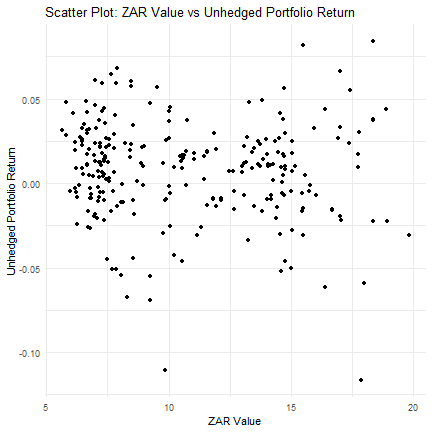
\includegraphics{Question-2_files/figure-latex/Figure 1-1} 

}

\caption{Unhedged vs ZAR/USD scatter plot \label{Figure1}}\label{fig:Figure 1}
\end{figure}

\hypertarget{hedged-scatterplot}{%
\subsubsection{Hedged scatterplot}\label{hedged-scatterplot}}

The findings of the hedged portfolio like that of the unhedged
portfolio, find a negative relationship between the ZAR/USD exchange
rate and the hedged portfolio returns. Which again is inline with the
findings of the study mentioned in the question.

\begin{figure}[H]

{\centering 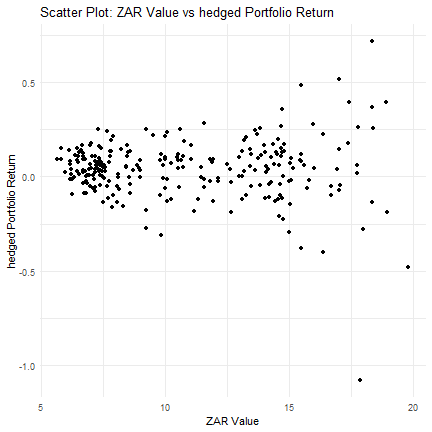
\includegraphics{Question-2_files/figure-latex/Figure 2-1} 

}

\caption{hedged vs ZAR/USD scatter plot \label{Figure2}}\label{fig:Figure 2}
\end{figure}

From the analysis completed above it is evident that there is a case for
not applying long-term (systematic) currency hedging to your portfolio.
To further unpack this statement I dive into my own analysis.

\hypertarget{own-study}{%
\subsection{Own study}\label{own-study}}

In this section of the question I dive into my own study. I evaluate a
comparison between the volatility of a hedge vs unhedged portfolio.

\hypertarget{comparison-of-hedged-vs-unhedged-portfolio-returns}{%
\subsection{Comparison of Hedged vs Unhedged Portfolio
Returns}\label{comparison-of-hedged-vs-unhedged-portfolio-returns}}

TO start of this comparison I first run a line graph showing the returns
of the hedged portfolio vs the returns of the unhedged portfolio. The
results further strengthen the statements made prior that the hedged
portfolio returns induce greater volatility than that of the unhedged
portfolio. To further unpack this discussion on volatility comparison I
use the PerformanceAnalytics package in R to fully evaluate the
volatility of the portfolios in question.

\begin{figure}[H]

{\centering 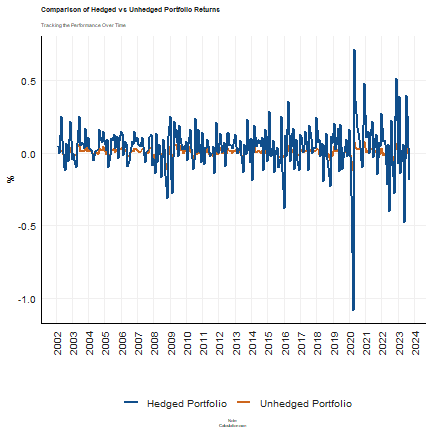
\includegraphics{Question-2_files/figure-latex/Figure 3-1} 

}

\caption{hedging comparisson plot \label{Figure3}}\label{fig:Figure 3}
\end{figure}

\hypertarget{understanding-the-volatility-of-the-hedged-vs-unhedged-portfolios}{%
\subsection{Understanding the volatility of the hedged vs unhedged
portfolios}\label{understanding-the-volatility-of-the-hedged-vs-unhedged-portfolios}}

In this section I calculate the rolling volatility and plot the results
for the hedged vs unhedged portfolios. To further the analysis I
evaluate a rolling period of 1 year with one of 3 years.

\hypertarget{calculating-the-rolling-volatility}{%
\subsubsection{Calculating the rolling
volatility}\label{calculating-the-rolling-volatility}}

Using the performance analytics package in R I am able to calculate the
1 year rolling volatility.

\hypertarget{rolling-realized-volatility-hedged-vs-unhedged-portfolio-plot}{%
\subsubsection{Rolling Realized Volatility: Hedged vs Unhedged Portfolio
plot}\label{rolling-realized-volatility-hedged-vs-unhedged-portfolio-plot}}

Here I plot a comparison of the rolling 1 year realized volatility of
the hedged vs unhedged portfolio using a line graph. As expected the
hedged portfolio continues to be accompanied by higher volatility
compared to that of the unhedged portfolio. To evaluate whether this is
just the case with the 1 year rolling volatility I evaluate the 3 year
rolling volatility next.

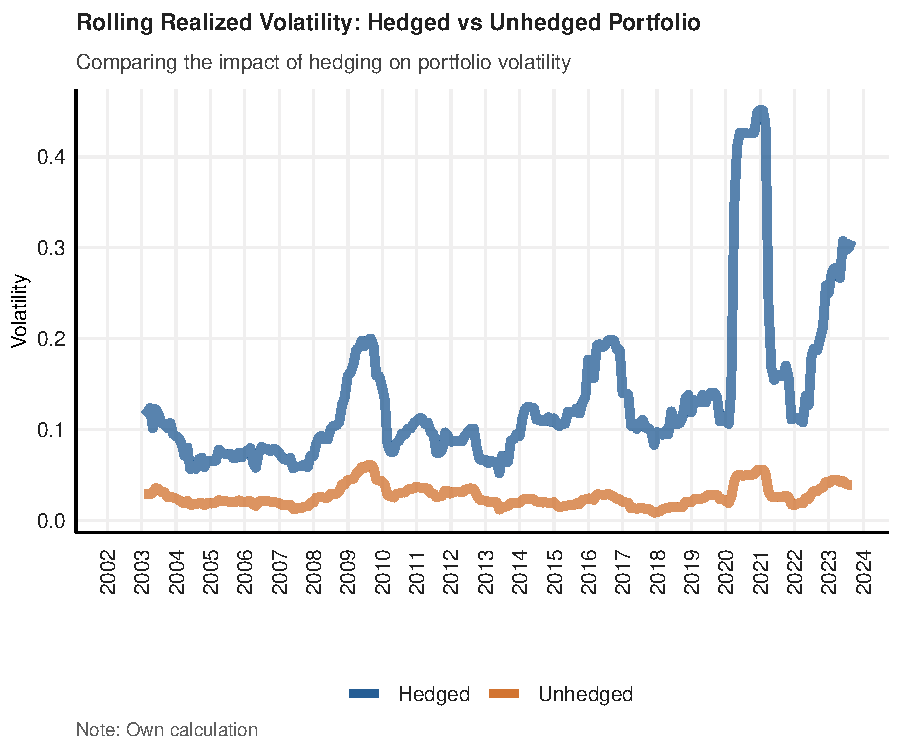
\includegraphics{Question-2_files/figure-latex/unnamed-chunk-6-1.pdf}

\hypertarget{lets-now-consider-a-longer-rolling-term-of-three-years-and-evaluate-its-impact-on-valatility}{%
\subsection{Lets now consider a longer rolling term of three years and
evaluate its impact on
valatility}\label{lets-now-consider-a-longer-rolling-term-of-three-years-and-evaluate-its-impact-on-valatility}}

Now considering a longer rolling term of three years I evaluate whether
the hedged portfolio still contains higher volatility compared to that
of the unhedged portfolio.

\hypertarget{calculating-rolling-volatility-using-36-months}{%
\subsubsection{Calculating rolling volatility using 36
months}\label{calculating-rolling-volatility-using-36-months}}

I calculate the 3 year rolling volatility for both the hedged and
unhedged portfolios.

\hypertarget{year-rolling-realized-volatility-hedged-vs-unhedged-portfolio-plot}{%
\subsubsection{3 year rolling realized volatility: Hedged vs Unhedged
Portfolio
plot}\label{year-rolling-realized-volatility-hedged-vs-unhedged-portfolio-plot}}

By utilizing the same methods as was used in calculating the 1 year
rolling realized volatility I am able to calculate the three year
rolling realized volatility and plot the results.

Once again it is evident that the hedged portfolio contains higher
volatility and therefore risk than that of the unhedged portfolio. The 3
year rolling return results in lower volatility than that of the 1 year
rolling volatility for the portfolios which can be expected due to
increased time period.

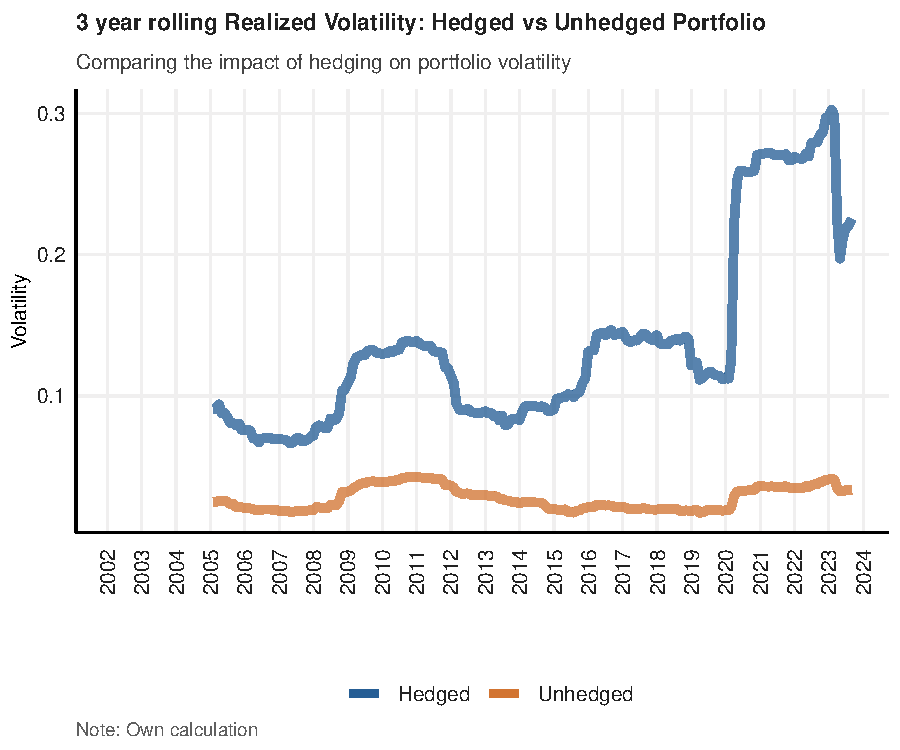
\includegraphics{Question-2_files/figure-latex/unnamed-chunk-8-1.pdf}

\hypertarget{conclusion}{%
\subsection{Conclusion}\label{conclusion}}

Thus, from the analysis completed above it is evident that the hedging
your portfolio to reduce risk may not be the appropriate way at tackling
risk. Hedging your portfolio may actually induce more volatility
resulting in higher risk.

\newpage

\hypertarget{references}{%
\section*{References}\label{references}}
\addcontentsline{toc}{section}{References}

\hypertarget{refs}{}
\begin{CSLReferences}{0}{0}
\end{CSLReferences}

\hypertarget{appendix}{%
\section*{Appendix}\label{appendix}}
\addcontentsline{toc}{section}{Appendix}

\hypertarget{appendix-a}{%
\subsection*{Appendix A}\label{appendix-a}}
\addcontentsline{toc}{subsection}{Appendix A}

Some appendix information here

\hypertarget{appendix-b}{%
\subsection*{Appendix B}\label{appendix-b}}
\addcontentsline{toc}{subsection}{Appendix B}

\bibliography{Tex/ref}





\end{document}
